\section{Instance Optimal Online Learning: Achievability via $\bob$} \label{sec:twoapprox}

Given the setting and problem statement above, we can now present the $\bob$ policy. 
We do this for a general online learning problem, wherein we want to combine $\ftl$ with any given algorithm $\wcalg$ with a worst-case regret guarantee $
\sup_{\ell^n} \Reg(\wcalg, \ell^n) \le g(n)
$. 
Before presenting the policy, we first need the following regret decomposition for $\ftl$. 
\begin{lemma}[Regret of $\ftl$] \label{lem:FTLRegret}
If $L_t(\cdot) \defeq \sum_{i=1}^t \ell_t(\cdot)$, i.e. the cumulative loss function, then
\begin{align*} 
    \Reg(\ftl, \ell^n) = \textstyle\sum_{t=1}^n (L_t(a^*_{t-1}) - L_t(a^*_t)). 
\end{align*}
\end{lemma}
This is reminiscent of the `be-the-leader' lemma~\citep{kalai2005efficient,slivkins2019introduction}, although never stated explicitly as an exact decomposition. 
\begin{proof}
Recall we define $\aftl_t = a^*_{t-1}$, and hence $\inf_{a \in \Ac} \sum_{t=1}^n \ell_t(a)= L_n(a^*_n) $. Now we have 
    \begin{align*}
        \Reg(\ftl, \ell^n) 
        &= \textstyle\sum_{t=1}^n \ell_t(a^*_{t-1})  - L_n(a^*_n) \\
        &= \textstyle\sum_{t=1}^n (L_t(a^*_{t-1}) - L_{t-1}(a^*_{t-1})) -  L_n(a^*_n) \\
        &= \textstyle\sum_{t=1}^n (L_t(a^*_{t-1}) - L_t(a^*_t)) + \textstyle\sum_{t=1}^n (L_t(a^*_t) - L_{t-1}(a^*_{t-1})) - L_n(a^*_n) \\
        &\stackrel{(a)}{=} \textstyle\sum_{t=1}^n (L_t(a^*_{t-1}) - L_t(a^*_t))
    \end{align*}
    where $(a)$ follows since $\sum_{t=1}^n (L_t(a^*_t) - L_{t-1}(a^*_{t-1})) = L_n(a^*_n)$ by telescoping. 
\end{proof}
Next, let $\ftlsum_t$ denote the \emph{anytime} regret that $\ftl$ incurs up to round $t$ (i.e., assuming the game ends after round $t$). From Lemma~\ref{lem:FTLRegret} we have
\begin{align} 
\label{eq:FTLRegEquality}
 \ftlsum_t \defeq \Reg(\ftl, \ell^t) = \textstyle\sum_{i=1}^t (L_i(a^*_{i-1}) - L_i(a^*_i)) 
\end{align}
Now we make three critical observations: 
\begin{itemize}
    \item $\ftlsum_t$ is \textbf{adapted}: it can be computed at the end of the $t^{th}$ round %after $\ell_t$ has been revealed, 
    \item $\ftlsum_t$ is \textbf{monotone} non-decreasing in $t$ (since by definition $L_i(a^*_{i-1}) - L_i(a^*_i) \ge 0$)
    \item $\ftlsum_t$ is an \textbf{anytime lower bound} for $\Reg(\ftl,\ell^n)$, with $\ftlsum_n = \Reg(\ftl, \ell^n)$
\end{itemize}
For an input threshold $\theta \ge 0$ and an algorithm $\wcalg$, we get the following (meta)algorithm.

\begin{algorithm}[ht] 
\label{alg:bob}
\SetAlgoNoLine
\caption{Switching via Monotone Adapted Regret Traces ($\bob$)}
\label{alg:bob}
\KwIn{Policies $\ftl, \wcalg$, threshold $\theta$} 
\textbf{Initialize} $\ftlsum_0=0$, $t=1$ \;
\While{$\ftlsum_{t-1} \le \theta$}
{
    Set $a_t = a_{t-1}^{*}$%
         \tcp*{Play $\ftl$}
    Observe $\ell_t(\cdot)$\; 
    Update $L_t(\cdot)=L_{t-1}(\cdot)+\ell_t(\cdot)$ and $\ftlsum_t=\ftlsum_{t-1}+(L_t(a_{t-1}^{*})-L_t(a_{t}^{*}))$ and $t = t+1$\;
}
Reset losses to $0$ and play $\wcalg$ for remaining rounds (See~\cref{fig:proof_intuition}(b)) \;
\end{algorithm}

% \begin{tcolorbox}[size=title]
% \label{alg:bob}
% \begin{center} \textbf{Algorithm 1:} Switching via Monotone Adapted Regret Traces ($\bob$)
% \end{center}
% \textbf{Input}: Policies $\ftl, \wcalg$, threshold $\theta$\\
% \textbf{Initialize} $\ftlsum_0=0$, $t=1$\\ 
% \textbf{While} $\ftlsum_{t-1} \le \theta$ \textbf{do}\\
% -- Set $a_t = a_{t-1}^{*}$; observe $\ell_t(\cdot)$\
%          \hfill\texttt{(Play $\ftl$)}\\
% -- Update $L_t(\cdot)=L_{t-1}(\cdot)+\ell_t(\cdot)$, $\ftlsum_t=\ftlsum_{t-1}+(L_t(a_{t-1}^{*})-L_t(a_{t}^{*}))$ and $t = t+1$\\
% \textbf{End}\\
% Reset losses to $0$ and play $\wcalg$ for remaining rounds (See~\cref{fig:proof_intuition}(b)).
% \end{tcolorbox}
%Given an regret upper bound guarantee of $g(n)$ on the performance of $\wcalg$, we show that $\bob$ with $\theta=g(n)$ is instance optimal with respect to the regret of $\ftl$ and the bound $g(n)$, achieving competitive ratio of 2.
We now have the following performance guarantee for Algorithm~\ref{alg:bob} for $\theta=g(n)$.
\begin{theorem}[Regret of $\bob$ with deterministic threshold]  
\label{thm:2ApproxRegret}
      We are given $\ftl$, and any other policy $\wcalg$ with worst-case regret $\sup_{\ell^n} \Reg(\wcalg, \ell^n) \le g(n)$
      for some monotone function $g$. Then, playing $\bob$ with threshold $\theta = g(n)$ ensures 
    \begin{align} \label{eq:2ApproxReg}
        \Reg(\bob, \ell^n) \le 2 \min\{\Reg(\ftl,\ell^n),g(n)\} + 1.
    \end{align}
\end{theorem}

%\begin{remark}[Competitive ratio] \label{rem:2CR}
%Another way of stating~\cref{thm:2ApproxRegret} is to say that it achieves a competitive ratio (CR) of 2 when compared against the $\ftl$ regret as well as the worst-case regret bound $g(n)$. 
%We will later improve this CR via a randomized switching rule. 
%\end{remark}
As we mention before, the structure of the $\bob$ algorithm (and the resulting guarantee) parallels the standard 2-competitive guarantee for the \emph{ski-rental} problem~\citep{karlin1994competitive}. 
This is a classical optimal stopping problem, where a principal faces an unknown horizon, and in each period must decide whether to rent a pair of skis for the period (for fixed cost \$1) or buy the skis for the remaining horizon (for fixed cost \$$B$). The aim is to design a policy which is minimax optimal (over the unknown horizon) with regards to the ratio of the cost paid by the principal, and the optimal cost in hindsight. 
%One can see that the optimal (deterministic) action to take for this problem is to rent the skis for $B-1$ days, buying on the $B-$th day to incur a total cost of $2B-1$. On the other hand, the hindsight optimal action for this instance would have been to buy the skis for $B$ cost upfront, leading to the decision-maker incurring a competitive ratio of 2.
%To see the analogy between the ski-rental problem and $\bob$, we observe that $\ftl$ mirrors the $\mathsf{rent}$ action, paying a cost of $L_t(a^*_{t-1}) - L_t(a^*_t)$ on day $t$ (see~\eqref{eq:FTLRegEquality}), and $\cover$ (or any $\wcalg$) mirrors the $\mathsf{buy}$ action, leading to the algorithm paying a cost of $g(n-t_{\mathrm{sw}})$ (where $t_{\mathrm{sw}}$ is the point at which $\bob$ switches from $\ftl$ to $\Cover$) after switching to the worst-case algorithm\footnote{While a strict equivalence to ski-rental would require paying a fixed cost of $g(n)$ after the $\mathsf{buy}$ action, in the worst instances we will have $t_{\mathrm{sw}} = o(n)$ so that $g(n-t_{\mathrm{sw}}) = g(n)(1+o(1))$}.
%The factor $2$ above is connected to the minimax-optimal deterministic policy for ski-rental.
We further expand on this connection in~\cref{ssec:binary} for the case of binary prediction. However, the connection suggests a natural follow-up question of whether randomized switching can help (as is the case for ski-rental); the following result answers this in the affirmative.
%Since it is well-known that employing algorithms with a  \emph{randomized} switching point between $\mathsf{rent}$ and $\mathsf{buy}$ can improve the competitive ratio for ski-rental, this suggests a natural randomized choice of $\theta$ in $\bob$ which leads to the following result


\begin{theorem}[Regret of $\bob$ with Randomized Thresholds]  
\label{thm:SkiRentalRegret}
We are given $\ftl$ and any other policy $\wcalg$ with worst-case regret $\sup_{\ell^n} \Reg(\wcalg, \ell^n) \le g(n)$
for some monotone function $g$. 
%Further, define cumulative density function $F_n(x) = \frac{e^{x/g(n)}-1}{e-1}$ for $x\in [0,g(n)]$. 
Moreover, given random sample $U\sim\text{Unif}[0,1]$, suppose we set
      \begin{align*}
      \theta=g(n)\ln(1+(e-1)U)
      \end{align*}
      Then playing the $\bob$ policy (Algorithm \ref{alg:bob}) with random threshold $\theta$ ensures 
    \begin{align*} 
    %\label{eq:eApproxReg}
        \E_{\theta}&\left[\Reg(\bob, \ell^n)\right]
        \le \frac{e}{e-1} \min\{\Reg(\ftl,\ell^n),g(n)\} + 1.
    \end{align*}
\end{theorem}
While we state the above as a randomized switching policy, this is more for interpretability -- it is easier to view our policy as switching between two black-box algorithms rather than playing a convex combination of the two. However, since we define the loss incurred by any $\alg$ in round $t$ to be the expected loss when $\alg$ plays a distribution $w_t$ over actions $\Ac$ (see~\cref{ssec:mainresults}), therefore we can alternately implement the above by mixing between the actions of $\ftl$ and $\wcalg$. More specifically, the above policy induces a \emph{monotone} mixing rule, where over $t$, the weight on the action suggested by $\wcalg$ is non-decreasing.

\begin{remark}[Optimality over Monotone Mixing Policies] 
\label{rem:SkiRentalLB}
The competitive ratio of $\frac{e}{e-1}$ is known to be optimal for the ski-rental problem via Yao's minmax theorem~\citep{borodin2005online}. A direct corollary of this is the optimality of $\bob$ over algorithms that are single switch (i.e., where the weight on $\wcalg$ is non-decreasing in $t$). One difference between our setting and ski-rental is that switching back-and-forth between $\ftl$ and $\wcalg$ is possible; see for example the $\mathsf{FlipFlop}$ policy of~\cite{de2014follow}. In~\cref{sec:converse} we provide a fundamental lower bound of $1.43$ on the competitive ratio over \emph{all} algorithms; this suggests that multiple switching can help get a better competitive ratio (since $e/(e-1)\approx 1.58$), but also, that single-switch policies are surprisingly close to optimal.
\end{remark}

\subsection{Illustrating the Reduction to Ski Rental in Binary Prediction}
\label{ssec:binary}

Before proving~\cref{thm:2ApproxRegret,thm:SkiRentalRegret}, we first illustrate the basic idea of our approach and reduction for the binary prediction setting. This is aided by the observation that the regret of $\ftl$ in this setting admits a simple geometric interpretation: for any sequence, and any time $t$, we have that $\ftlsum$ is equal to 1/2 times the number of `lead changes' up to time $t$; where a lead change is a time step $i$ where the count of $1$s and $0$s in the (sub)sequence $y^{i-1}$ is equal (see Figure~\ref{fig:proof_intuition}(a)). 
%i.e. rounds at which the total number of 0s and 1s are equal. 
\begin{corollary}[$\ftl$ for binary prediction] \label{cor:BinPred}
In binary prediction, for any sequence $y\in\{0,1\}^n$ and any time $t\leq n$, define the lead-change counter
\[
c(y^t) \defeq |\{0 \le j \le t ~s.t.~ \sum_{i=1}^j y_i = \sum_{i=1}^j (1-y_i)\}|.
\]
Then we have $\ftlsum_t = \frac12 c(y^{t-1})$ and thus $\Reg(\ftl, y^n) = \frac12 c(y^{n-1})$. 
\end{corollary}

Corollary \ref{cor:BinPred} follows from the regret decomposition in Lemma \ref{lem:FTLRegret}. Furthermore, since the losses of 0s and 1s are equal at a lead change, it also follows that at a lead change $t$, the anytime regret $\ftlsum_t$ is also equal to the hindsight regret incurred by $\ftl$ up to time $t$. Since $\ftlsum_t$ only increases in value at lead changes, if the $\bob$ algorithm switches to $\wcalg$, it will only happen after a lead change, and thus $\bob$ behaves as if it had oracle knowledge of the regret of $\ftl$ from just the history up to the current time.

Consider the instantiation of $\bob$ where $\wcalg = \cover$ and $g(n) = \sqrt{\frac{n}{2 \pi}}$. As mentioned in Section~\ref{sec:intro}, a remarkable property of $\cover$ is that it is the true minimax optimal algorithm, where $\Reg(\Cover,y^n) = \sqrt{\frac{n}{2 \pi}} (1+o(1))$ for all sequences $y^n$, such that $g(n)$ is nearly equal to $\Reg(\Cover,y^n)$ regardless of the sequence~\citep{Cover1966}. 

It follows that $\bob$ is equivalent to an algorithm which starts with $\ftl$, plays it until the regret of $\ftl$ matches the minimax regret guaranteed by $\cover$ for the remaining sequence, and then switches to $\cover$ until the end. 
Let $t_{\mathrm{sw}}$ denote the last round $\bob$ plays $\ftl$ before switching to $\wcalg$ (with $t_{\mathrm{sw}}=n$ if it never switches).
For a single switch algorithm, the sequence which maximizes the regret is one that maximizes the $\ftl$ regret before the switch at $t_{\mathrm{sw}}$, and minimizes the $\ftl$ after the switch, as depicted in Figure \ref{fig:proof_intuition}(a). For such a sequence, $\ftlsum_t = t/4$ at lead changes $t$, such that the regret incurred by the algorithm is linear before the switch, matching the linear cost of renting skis in the ski rental problem. Note that $t_{\mathrm{sw}}$ will necessarily be $o(n)$ in such sequences as the time it takes until $\ftlsum_t \geq g(n)$ is linear in $g(n) = o(n)$. After the switch, $\cover$ will incur regret $\sqrt{\frac{n-t_{\mathrm{sw}}}{2 \pi}} (1+o(1)) = g(n) (1 + o(1))$, matching the fixed cost of buying skis at the switching point; Corollary \ref{cor:binary_pred_guarantees} follows as a result of this analysis. Furthermore, in the binary prediction setting, $\bob$ achieves the stronger notion of instance optimality stated in Definition \ref{def:instanceopt_binary}.

\begin{corollary} \label{cor:binary_pred_guarantees}
For all $y^n\in\{0,1\}^n$, $\bob$ with $\wcalg=\cover$ and $\theta = \sqrt{\frac{n}{2 \pi}}$ satisfies
\begin{align*}
    \Reg(\bob,y^n) &\leq 2\min\{\Reg(\ftl,y^n),\Reg(\cover,y^n)\} + 1.
\end{align*}
$\bob$ with $\wcalg=\cover$ and $\theta = \sqrt{\frac{n}{2\pi}}\ln(1+(e-1)U)$ for $U\sim\text{Uniform}[0,1]$ satisfies
\begin{align*}
    \Reg(\bob,y^n)
    &\leq 1.58\min\{\Reg(\ftl,y^n),\Reg(\cover,y^n)\} + 1.
\end{align*}
\end{corollary}
%\cycomment{I don't know if it's worth stating again, but I think it's worth commenting that in binary prediction, we get the stronger type of instance optimality since regret of cover is equal to the regret upper bound.}

\begin{figure}[!t]
  \begin{minipage}{0.3\textwidth} % Adjust the width as needed
    \centering
    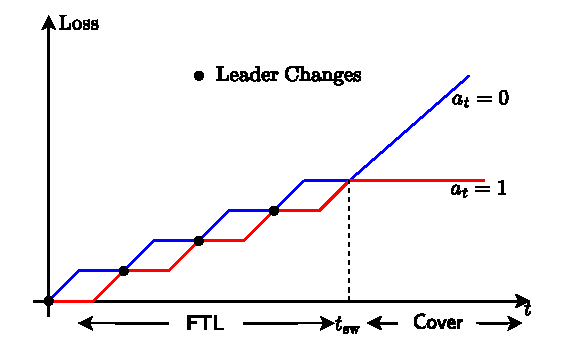
\includegraphics[height=\linewidth]{figures/LeaderChangesBinary.pdf}
  \end{minipage}%
  \hspace{1in}
  \begin{minipage}{.37\textwidth} % Adjust the width as needed
    \centering
    \vspace{1.3em}
    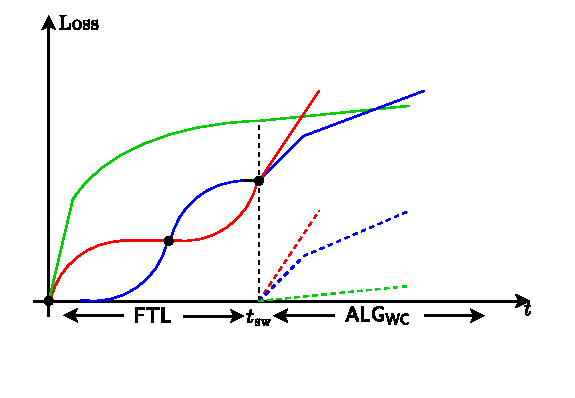
\includegraphics[height=\linewidth]{figures/ExpertsReset.pdf}
  \end{minipage}%
\captionsetup{format=plain}
  \vspace{-0.5em}\caption{\it\footnotesize Figure \ref{fig:proof_intuition}(a) on the left shows the worst case instance in binary prediction for an algorithm which starts with $\ftl$ and switches at most once during the time horizon to $\cover$. Figure\ref{fig:proof_intuition}(b) on the right depicts in a prediction with experts setting how $\bob$ resets the losses after the switch from $\ftl$ to $\wcalg$.}
  \label{fig:proof_intuition}
  \vspace{-0.5cm}  
\end{figure}

% A corollary of our result specialized to binary prediction is the following:
% \begin{corollary}
% Define $C_0=1$, $C_t=C_{t-1}+\mathds{1}_{[\sum_{i\leq t}y_i=t/2]}$, and $\theta=\sqrt{\frac{n}{2\pi}}\ln(1+(e-1)U)$ where $U\sim\text{Uniform}[0,1]$. Let $\bob$ be the policy which follows $\ftl$ if $C_t<\theta$, else switches to $\cover$. Then $\forall\,y^n\in\{0,1\}^n$: 
% \begin{align*}
%     \Reg(\bob,y^n)
%     &\leq 1.58\min{\Reg(\ftl,y^n),\Reg(\cover,y^n)}.
% \end{align*}
% \end{corollary}

% % To understand how this is achieved, consider a thought experiment of the oracle who knows beforehand which of $\ftl$ and $\cover$ is better on input $y^n$. As we mention, the challenge in matching this oracle is that to compute the regret of an algorithm, we need to know the best action in hindsight. However, an important observation is that for $\ftl$, at any $t\in[n]$, there is an estimator $\ftlsum_t$ that:\\
% % $(i)$ is \emph{adapted} (and hence computable) from history,\\ 
% % $(ii)$ is \emph{monotone}, i.e., non-decreasing with $t$, and \\
% % $(iii)$ is a \emph{lower bound} for $\Reg(\ftl,y^n)\,\forall\,t\in[n]$.\\
% While this result is established generally in Lemma~\ref{lem:FTLRegret}, we see that in binary prediction the $\ftl$ regret admits a geometric interpretation as $\ftlsum_t = C_t/2$, where $C_t$ is the number of rounds before $t$ when the number of $0$s equals the number of $1$s. On the other hand, a worst-case optimal policy like $\cover$ for binary prediction comes equipped with an upper bound $g(n)$ on its regret over \emph{any} input of length $n$. 

% % \begin{figure}[!t]
% %   \centering
% %   \begin{minipage}{.3\textwidth} % Adjust the width as needed
% %     \centering
% %     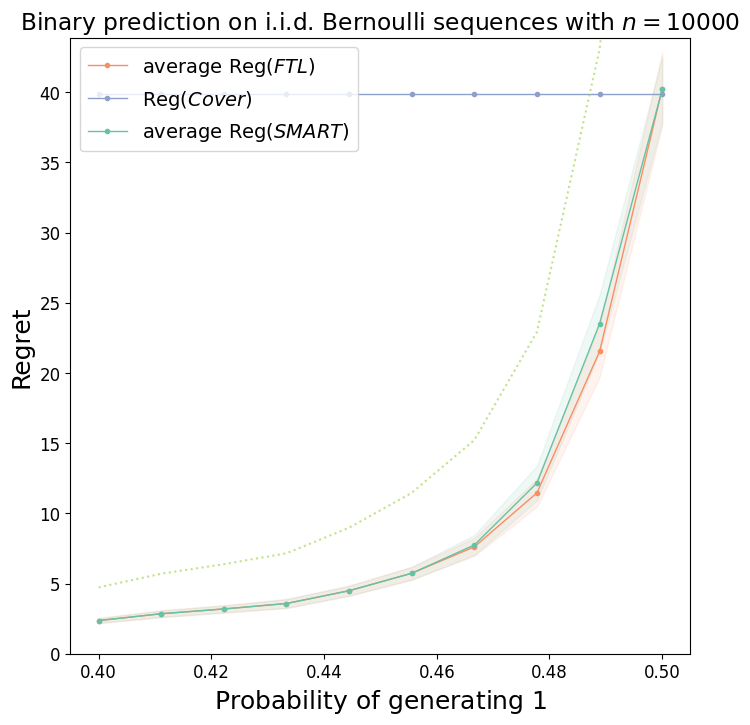
\includegraphics[height=\linewidth]{figures/detSMART_iid.png}
% %     %\caption{\it\scriptsize (a) $\bob$ with deterministic $\theta$, i.i.d. $y^n$}
% %   \end{minipage}%
% %   \hfill
% %   \begin{minipage}{.3\textwidth} % Adjust the width as needed
% %     \centering
% %     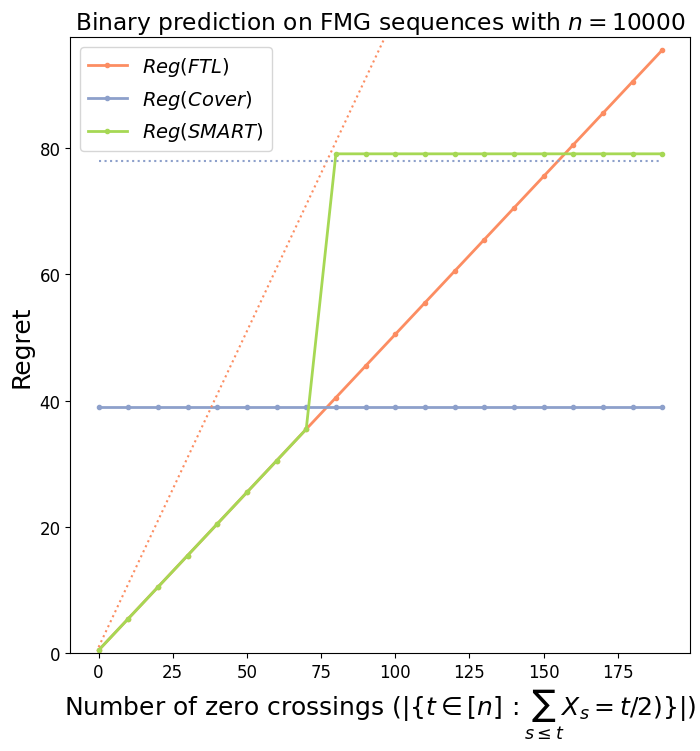
\includegraphics[height=\linewidth]{figures/detSMART_FMG.png}
% %     %\caption{\it\scriptsize (b) $\bob$ with deterministic $\theta$: FMG $y^n$}
% %   \end{minipage}%
% %   \hfill
% %   \begin{minipage}{.3\textwidth} % Adjust the width as needed
% %     \centering
% %     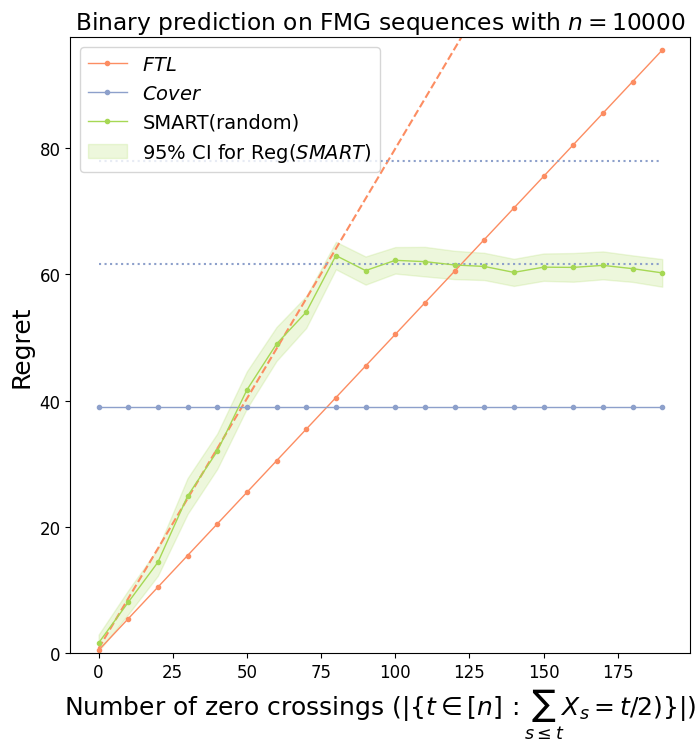
\includegraphics[height=\linewidth]{figures/randomSMART_FMG.png}
% %     %\caption{\it\scriptsize (c) $\bob$ with randomized $\theta$, FMG $y^n$}
% %   \end{minipage}
% % \captionsetup{format=plain}
% %   \caption{\it\footnotesize Comparing regret of $\ftl$, $\cover$ and $\bob$ on a collection of input sequences (for fixed $n$).\\ 
% %   $\bullet$ In Fig. $(a)$, we consider i.i.d. Bernoulli$(p)$ inputs for varying $p$. The regret of $\ftl$ is much lower than $\cover$ for $p<1/2$; the regret of $\bob$ tracks $\ftl$ closely (better than $2\Reg(\ftl)$, indicated by dotted line).\\
% %   $\bullet$ In Fig. $(b)$ and $(c)$, we consider `worst-case' binary sequences (as per~\citep{feder1992universal}) parameterized by the number of `$0$-crossings': the sequence with parameter $c$ comprises of $c$ pairs `$0,1$' or `$1,0$', followed by $n-2c$ `$1$'s. 
% %   %$\Reg(\ftl)$ on the sequence with $c$-crossings is $c/2$, while $\Reg(\cover)$ is constant ($\approx\sqrt{\frac{n}{2 \pi}}$). 
% %   In Fig. $(b)$, we consider $\bob$ with a deterministic switching threshold (\cref{thm:2ApproxRegret}) and compare $\Reg(\bob)$ with $2\Reg(\ftl)$ and $2\Reg(\cover)$ (dotted lines); in Fig. $(c)$, we use a randomized threshold (\cref{thm:SkiRentalRegret}), and show the average regret over the randomized threshold, as well as sample paths (plotted in green), and compare with $\frac{e}{e-1}$ times $\Reg(\ftl)$ and $\Reg(\cover)$ (dotted lines).}
% %   \label{fig:SMART}
% %   \vspace{-0.5cm}  
% % \end{figure}
% We illustrate this result in~\cref{fig:SMART}, comparing the regret of $\bob$ (both with randomized thresholds as stated above, and also with deterministic threshold $\theta=\sqrt{2n/\pi}$) to that of $\ftl$ and $\cover$. Fig.$(a)$ shows that on stochastic inputs, $\Reg(\bob)$ is almost the same as $\Reg(\ftl)$ and far below $\Reg(\cover)$. Figs.$(b)$ and $(c)$ indicate that this is not always true; however, $\bob$ still tracks the better of $\ftl$ and $\cover$ up to a constant factor ($2$ for deterministic, $1.58$ for randomized). Note this holds \emph{on every sequence} -- in particular, while we average across sequences in Fig.$(a)$ to show the trend, in Figs.$(b)$ and $(c)$ the regret is measured on a single sequence for each data point. 
% %Thus, $\bob$ is indeed instance-optimal.

\subsection{Proofs for General Online Learning}

In the general online learning setting, the proof is nearly the same, with the reduction to the ski-rental problem captured by Lemma \ref{lemma:regret_skirental}.
\begin{lemma} \label{lemma:regret_skirental}
Let $t_{\mathrm{sw}} \defeq \min_{1 \le t \le n-1} \ftlsum_t > \theta$ denote the last round $\bob$ plays $\ftl$ before switching to $\wcalg$ (with $t_{\mathrm{sw}}=n$ if it never switches). $\bob$ incurs regret bounded by
\[\Reg(\bob, \ell^n) \leq \Reg(\ftl, \ell^{t_{\mathrm{sw}}}) + \Reg(\wcalg, \ell_{t_{\mathrm{sw}}+1}^n) \leq \theta + \Reg(\wcalg, \ell_{t_{\mathrm{sw}}+1}^n) + 1.\]
\end{lemma}

\begin{proof}
We separately bound the regret of $\bob$ before the switch and after the switch,
\begin{align*}
\Reg(\bob, \ell^n)
%&= \textstyle\sum_{t=1}^t_{\mathrm{sw}} \ell_t(a_t) + \textstyle\sum_{t = t_{\mathrm{sw}}+1}^n \ell_t(a_t) - \textstyle\sum_{t=1}^n \ell_t(a^*_n) \\
&=  \big(\textstyle\sum_{t=1}^{t_{\mathrm{sw}}} \ell_t(a_t) - \textstyle\sum_{t=1}^{t_{\mathrm{sw}}} \ell_t(a^*_n)\big) + \big(\textstyle\sum_{t=t_{\mathrm{sw}}+1}^n \ell_t(a_t) - \textstyle\sum_{t=t_{\mathrm{sw}}+1}^n \ell_t(a^*_n)\big) \\
&\stackrel{(a)}{\le} \big(\textstyle\sum_{t=1}^{t_{\mathrm{sw}}} \ell_t(a_t) - \textstyle\sum_{t=1}^{t_{\mathrm{sw}}} \ell_t(a^*_{t_{\mathrm{sw}}})\big) + \big(\textstyle\sum_{t=t_{\mathrm{sw}}+1}^n \ell_t(a_t) - \textstyle\sum_{t=t_{\mathrm{sw}}+1}^n \ell_t(a^*_{t_{\mathrm{sw}}+1:n})\big) \\
&= \Reg(\ftl, \ell^{t_{\mathrm{sw}}}) + \Reg(\wcalg, \ell_{t_{\mathrm{sw}}+1}^n).
\end{align*}
The first term is upper bounded by $\Reg(\ftl, \ell^{t_{\mathrm{sw}}})$ since $L_{t_{\mathrm{sw}}}(a^*_n) \ge L_{t_{\mathrm{sw}}}(a^*_{t_{\mathrm{sw}}})$ by definition, as $a^*_{t_{\mathrm{sw}}}$ is the minimizer of $L_{t_{\mathrm{sw}}}$, and furthermore $\bob$ always plays according to $\ftl$ in rounds up to $t_{\mathrm{sw}}$. The second term is upper bounded by $\Reg(\wcalg, \ell_{t_{\mathrm{sw}}+1}^n)$ because $\sum_{t=t_{\mathrm{sw}}+1}^n \ell_t(a^*_{t_{\mathrm{sw}}+1:n}) \leq \sum_{t=t_{\mathrm{sw}}+1}^n \ell_t(a^*_n)$ as $a^*_{t_{\mathrm{sw}}+1:n}$ is the minimizer of the losses after $t_{\mathrm{sw}}$, and at time $t > t_{\mathrm{sw}}$, $\bob$ plays according to $\wcalg$ on the sequence of losses limited to $\ell_{t+1}^n$. This illustrates the important role of resetting the losses after the switch as depicted in Figure \ref{fig:proof_intuition}(b).
Using the fact that $\ftlsum_{t_{\mathrm{sw}}-1} \le \theta$ and $L_{t_{\mathrm{sw}}-1}(x^*_{t_{\mathrm{sw}}-1}) \le L_{t_{\mathrm{sw}}-1}(x^*_{t_{\mathrm{sw}}})$, it follows that \\
$~~~~~~\Reg(\ftl, \ell^{t_{\mathrm{sw}}}) = \ftlsum_{t_{\mathrm{sw}}-1} + L_{t_{\mathrm{sw}}-1}(a^*_{t_{\mathrm{sw}}-1}) - L_{t_{\mathrm{sw}}-1}(x^*_{t_{\mathrm{sw}}}) + \ell_{t_{\mathrm{sw}}}(a^*_{t_{\mathrm{sw}}-1}) - \ell_{t_{\mathrm{sw}}}(x^*_{t_{\mathrm{sw}}}) \leq \theta + 1.$
\end{proof}

The reduction to ski-rental is again immediate due to the properties that $\ftlsum_t := \Reg(\ftl,\ell^{t_{\mathrm{sw}}})$ is adapted, monotone, and is an anytime lower bound for $\Reg(\ftl,\ell^n)$, while remaining an upper bound on the true regret incurred by $\ftl$ up to time $t$. As a result, the algorithm can pretend that it truly observes the regret it incurs at each time up to the switching time $t_{\mathrm{sw}}$. After the switch, $\bob$ incurs regret $\Reg(\wcalg, \ell_{t_{\mathrm{sw}}+1}^n)$ which is upper bounded by $g(n-t_{\mathrm{sw}}) \leq g(n)$ by assumption.\\

% \begin{metaalg}[Threshold$(n), \wcalg$] 
%\label{metaalg:2approx}
% \end{metaalg}
%     \noindent\fbox{%
%     \parbox{0.95\textwidth}{%
%         \begin{itemize}
%             \item Play the  action as long as $\ftlsum_t \le \text{Threshold}(n)$ 
%             \item Let $t_{\mathrm{sw}} \defeq \min_{1 \le t \le n-1} \ftlsum_t >$ Threshold$_n$. Starting from $t = t_{\mathrm{sw}}+1$, forget $\ell^{t_{\mathrm{sw}}}$ and start playing $\wcalg$. 
%         \end{itemize}
%     }%
% }

\begin{proof}[Proof of Theorem~\ref{thm:2ApproxRegret}]
This follows immediately from Lemma \ref{lemma:regret_skirental}. For $\ell^n$ such that $\Reg(\ftl,\ell^n) \le g(n)$, $\bob$ will never switch to $\cover$ as $\ftlsum_t \le \Reg(\ftl, \ell^n) \leq g(n)$ such that $\Reg(\bob,\ell^n) = \min\{\Reg(\ftl, \ell^n), g(n)\}$. For $\ell^n$ such that $\Reg(\ftl,\ell^n) > g(n)$, by Lemma \ref{lemma:regret_skirental}, $\Reg(\bob, \ell^n)\leq g(n) + g(n-t_{\mathrm{sw}}) +1 \leq 2 g(n) +1$. \\% by monotonicity of $g(\cdot)$.  \begin{flushright}$\blacksquare$\end{flushright}
\end{proof}

% \abedit{
% Let's take the simple case of binary prediction. We have, for a fixed threshold $\theta$ that (representing ftl regret by $r$ and worst-case regret by $g$) 
% \begin{align}
%     \Reg(\bob,y^n) = r \indi\{r \le \theta\} + (\theta+g) \indi\{r > \theta\}.
% \end{align}
% Therefore, we have 
% \begin{align*}
% \frac{\Reg(\bob,y^n)}{\min\{r,g\}} =  \begin{cases} 
%   \indi\{r \le \theta\} + \frac{\theta+g}{r} \indi\{r > \theta\} & \text{ if } r \le g \\
%       \frac{r}{g}\underbrace{\indi\{r \le \theta\}}_{=0 \text{ since } r \ge g \ge \theta} + \frac{\theta+g}{g} \underbrace{\indi\{r > \theta\}}_{= 1 \text{ again, since } r \ge g \ge \theta}    & \text{if } r \ge g
%   \end{cases}
% \end{align*}
% 

\begin{proof}[Proof of Theorem~\ref{thm:SkiRentalRegret}]
The proof uses a primal-dual approach, similar to that of~\cite{karlin1994competitive} for ski-rental.
For a given sequence of loss functions $\ell^n$, we use the shorthand $r= \Reg(\ftl,\ell^n)$ and $g=g(n)$.
Also, for our given choice of cumulative distribution function $F_n$, the corresponding probability density function is given by $f(z) = \frac{e^{z/g}}{g(e-1)}$ for $z\in[0,g]$. 
As before, let $t_{\mathrm{sw}} \defeq \min_{1 \le t \le n-1} \ftlsum_t > \theta$ be the (random) round where $\bob$ switches from $\ftl$ to $\wcalg$ (with $t_{\mathrm{sw}}=n$ if it never switches). Then by Lemma \ref{lemma:regret_skirental} we have
\begin{align*}
\frac{\Reg(\bob,\ell^n) -1}{\min\{\Reg(\ftl,\ell^n),g(n)\}}\leq \begin{cases} 
   \frac{\theta + g}{\min\{r,g\}} & \text{if } t_{\mathrm{sw}} < n \\
   1       & \text{if } t_{\mathrm{sw}} = n
  \end{cases}
\end{align*}
where the second case follows from the fact that $\theta\in[0,g]$, and hence if we never switch, then $r\le g(n)$. 
Taking expectation over $\theta$, we have
\begin{align*}
&\frac{\E_{\theta}\left[\Reg(\bob,\ell^n)\right]-1}{\min\{\Reg(\ftl,\ell^n),g\}}
\le 
\begin{cases} 
   \int_0^r   \frac{x + g}{r}f(x)dx + 1 - F(r)  & \text{if } r \le g \\
   \int_0^g   \frac{x + g}{g}f(x)dx        & \text{if } r > g
  \end{cases}
\end{align*}
Let $\phi(z) \defeq  \int_0^z \frac{(x + g)}{z}f(x)dx + 1 - F(z) $ for $z\in[0,g]$; then $\frac{\E_{\theta}\left[\Reg(\bob,\ell^n)\right]-1}{\min\{\Reg(\ftl,\ell^n),g\}} \leq \max_{z\in[0,g]}\phi(z)$. Moreover, we can differentiate to get $z^2\phi'(z)= gzf(z) - \int_0^z(x + g)f(x)dx$. Substituting our choice of $f$ in this expression, we get
\begin{align*}
\frac{z^2d\phi(z)}{dz} &= \frac{ze^{z/g}}{(e-1)} - \int_0^z(x + g)\frac{e^{x/g}}{g(e-1)}dx
=\frac{ze^{z/g} - g\int_0^{z/g}(w + 1)e^{w}dw}{(e-1)}=0
%\\&=\frac{ze^{z/g} - g(ze^{z/g}/g)}{(e-1)} = 0
\end{align*}
Thus, $\phi(z)$ is constant for all $z\in[0,g]$ and $\phi(g) = \frac{1}{g(e-1)}\int_0^g(1+x/g)e^{x/g}dx = \frac{e}{e-1}$. 
\end{proof}
%%%%%%%%%%%%%%%%%%%%%%%%%%%%%%%%%%%%%%%%%%%%%%%%%%%%%%%%%%%%%%%%%%%%%%%%%%%%%%%%%%%%%%%%%%%%%%%%%%%%%%%%%%%%%%%%%%%%%%%%%%%%%%%%%%%%%%%%%%%%%%%%%%%%%%%%%%%%%%%%%%%%%%
% \abdelete{
% \subsection{Examples} \label{subsec:examples2Approx}

% We now instantiate~\cref{alg:bob} in a few special cases. 

% \paragraph{FTL and Cover's algorithm:} In the setting of binary prediction, recall Cover's algorithm from~\cref{ssec:Cover} which chooses $\widehat{Y}_t = \Majority\{y^{t-1},\e_{t+1}^n\}$
%      where $\e_{t+1}^n \sim \mathrm{Bern}\left(\frac{1}{2}\right)$ i.i.d., with ties broken uniformly at random. 
%     %For any other $\alg$, 
%     % \[
%     % \max_{y^n} \Reg(\alg, y^n) \ge \max_{y^n} \Reg(\Cover, y^n)
%     % \].
% % \begin{theorem} \label{thm:CoverThm}
% % Let a function $\phi : \{0,1\}^n \to \mathbb{R}+$ be \emph{achievable} in binary prediction if there exists a predictor/strategy $a_t: y^{t-1} \mapsto [0,1]$ that achieves 
% % \begin{align}\label{eq:AchievabilityDefn}
% %     \sum_{t=1}^n |a_t(y^{t-1})-y_t| = \phi(y^n)
% % \end{align}
% % for all $y^n$. Then, the following are necessary conditions for a loss function to be achievable:
% % \begin{itemize}
% %     \item Balance: For $\e^n \sim \mathrm{Bern}\left(\frac{1}{2}\right)$ i.i.d., 
% %     \begin{align}\label{eq:BalanceCondn}
% %         \E[\phi(Y^n)] = \frac{n}{2} 
% %     \end{align}
% %     \item Stability: Let $\phi_t(y^t) \equiv \E[\phi(y^{t}\e_{t+1}^n)]$ where $\e_{t+1}^n \sim \mathrm{Bern}\left(\frac{1}{2}\right)$ i.i.d. Then
% %     \begin{align}\label{eq:StabilityCondn}
% %         |\phi_t(y^{t-1}0)-\phi_t(y^{t-1}1)| \le 1. 
% %     \end{align}
% %     Furthermore, if a function $\phi$ is satisfies the above two conditions, then the predictor 
% %     \begin{align} 
% %     a_t(y^{t-1}) = \frac{1+\phi_t(y^{t-1}0)-\phi_t(y^{t-1}1)}{2}
% %     \end{align}
% %     achieves it. 
% % \end{itemize}
% % \end{theorem}

% % A particularly illuminating question is whether the loss of the hindsight-optimal action, i.e. $\phi(y^n) = \min\{\sum_{t=1}^n y_i, n-\sum_{t=1}^n y_i\}$ is achievable, which is answered in the negative by Cover's result. 

% % \begin{corollary}\label{cor:BinPredOptReg}
% %     The loss function $y^n \mapsto \min\left\{\sum_{t=1}^n y_i, n-\sum_{t=1}^n y_i\right\}$ violates the balance condition and therefore is not achievable. However, the function 
% %     \begin{align}\label{eq:CoverLossFn}
% %     y^n \mapsto \min\left\{\sum_{t=1}^n y_i, n-\sum_{t=1}^n y_i\right\} + \frac{E|\sum_{t=1}^n Z_t|}{2}
% %     \end{align}
% %     where $Z^n \sim \Unif\{+1,-1\}$ i.i.d. is achievable. The predictor that achieves~\cref{eq:CoverLossFn} chooses $\widehat{Y}_t$ (equivalently, $a_t = \mathsf{P}[\widehat{Y_t} = 1]$)
% %     \begin{align}\label{eq:CoverPredictor}
% %         \widehat{Y}_t = \Majority\{y^{t-1},\e_{t+1}^n\}
% %     \end{align} 
% %     where $\e_{t+1}^n \sim \mathrm{Bern}\left(\frac{1}{2}\right)$ i.i.d., with ties broken uniformly at random. Finally, Cover's predictor~\cref{eq:CoverPredictor} is \emph{minmax optimal} in the sense that for any other predictor $\alg$, 
% %     \[
% %     \max_{y^n} \Reg(\alg, y^n) \ge \max_{y^n} \Reg(\Cover, y^n).
% %     \]
% % \end{corollary}
% %\cycomment{given AISTATS length, the above discussion about cover can be moved to appendix}
% Recall also that $\Reg(\Cover,y^n) = \frac12 \E\Big|\sum_{t=1}^n Z_t\Big| = \sqrt{\frac{n}{2\pi}}(1+o(1))$ i.e. Cover's predictor is an \emph{equalizer}. 
% Choosing $\wcalg$ to be $\Cover$ and $g(n) = \frac12 \E|\sum_{t=1}^n Z_t|$ in $\bob$ yields 
% \begin{align}
%     \Reg(\bob,y^n) \le %\frac{e}{e-1}\min\left\{\Reg(\ftl, y^n), g(n)\right\} + 1 =  
%     \frac{e}{e-1}\min\left\{\Reg(\ftl, y^n), \Reg(\Cover,y^n)\right\} \nonumber %\label{eq:BoBFTLCov}
% \end{align}
% Thus, SMART is able to match the \emph{instance-wise} regret achieved by the minimax optimal predictor in the stochastic case and the minimax optimal predictor in the individual-sequence case.

% \paragraph{FTL and Hedge:} \label{subsubsec:FTLHedge}
% In the setting of prediction with expert advice, the exponential weights or Hedge algorithm picks the action $a_t$ (for a learning rate $\eta$) $a_{tj} \propto \exp\big(-\eta \textstyle\sum_{i=1}^{t-1}\ell_{ij} \big)$.
% The regret guarantee for Hedge for learning rate $\eta = \sqrt{\frac{8 \ln m}{n}}$ is known to be~\cite[Theorem 2.2]{Cesa-Bianchi--Lugosi2006} $\max_{\ell^n} \Reg(\mathsf{Hedge},\ell^n)  \le \sqrt{\frac{n\ln m}{2}}$
% which implies that instantiating $\bob$ with $\wcalg$ to be $\mathsf{Hedge}$ and $g(n) = \sqrt{\frac{n \ln m}{2}}$ yields
% \begin{align*}%\label{eq:BoBFTLHedge}
%     \Reg(\bob, \ell^n) \le \frac{e}{e-1}\min\big\{\Reg(\ftl,\ell^n), \sqrt{\tfrac12 n \ln m}\big\}.
% \end{align*}
% We note that Hedge is asymptotically minimax optimal as $n, m \to \infty$, see~\cite[Theorem 3.7]{Cesa-Bianchi--Lugosi2006}.

% \paragraph{FTL and (known) small-loss algorithms:} \label{subsubsec:FTLSmallLoss}
% So far, we have achieved regret guarantees that match the better of the FTL regret and a worst-case \emph{upper bound} on the regret achieved by $\wcalg$ (as opposed to $\Reg(\wcalg, \ell^n)$). However, if $\wcalg$ is designed to be able to achieve low regret for benign sequences $\ell^n$, then it is desirable to match, if not exactly $\Reg(\wcalg, \ell^n)$, some upper bound that depends on $\ell^n$. If a bound on the loss incurred by the hindsight-optimal expert is known apriori, using $\bob$ achieves such a result.
% \begin{corollary}\label{cor:BOBWKnownLStar}
%     If $\min_{j\in [m]} \sum_{t=1}^n \ell_{tj} \le L^*$ for a known $L^*$ and the algorithm $\wcalg$ satisfies 
%     \[
%     \Reg(\wcalg, \ell^n) \le g\Big(\min_{j \in [m]} \textstyle\sum_{t=1}^n \ell_{tj}\Big)
%     \]
%     for all $\ell^n$ %\cycomment{satisfying the small loss condition} 
%     and monotone increasing $g(\cdot)$, then $\bob$ with $\wcalg$ and $g(L^*)$ achieves 
%     \begin{align*}
%         \Reg(\bob, \ell^n) \le \frac{e}{e-1}\min\{\Reg(\ftl, \ell^n), g(L^*)\} + 1 
%     \end{align*}
% \end{corollary}

% Note that the setting in Corollary~\ref{cor:BOBWKnownLStar} presumes knowledge of a good upper bound on the loss achieved by the best expert. In the next section, we provide an algorithm that circumvents this and achieves the guarantee in Corollary~\ref{cor:BOBWKnownLStar} with a larger competitive ratio.
% }



% \begin{proof}
%     The proof is almost identical to that of~\cref{thm:2ApproxRegret}, with the only change being that when $g(L^*) \ge \Reg(\ftl,\ell^n)$, then (recalling that $t_{\mathrm{sw}}$ denotes the switch point) 
%     \[
%     \Reg(\bob,\ell^n) \le g(L^*)+1+g\left(\min_{j}\sum_{t=t_{\mathrm{sw}}+1}^n \ell_{tj}\right) \le 2g(L^*) + 1
%     \]
%     since $\min_{j}\sum_{t=t_{\mathrm{sw}}+1}^n \ell_{tj} \le \min_{j}\sum_{t=1}^n \ell_{tj} \le L^*$ and $g(\cdot)$ is monotone.
% \end{proof}
%%%%%%%%%%%%%%%%%%%%%%%%%%%%%%%%%%%%%%%%%
%%%%%%%%%%%%%%%%%%%%%%%%%%%%
%\subsection{Experiments} \label{subsec:Expts}
%%%%%%%%%%%%%%%%%%%%%%%%%%%%%%%%%%%%%%%%%%%%%%%%%%%%%%%%%%%%%%%%%%%%%%%%%%%%%%%%%%%%%%%%%%%%%%%%%%%%%%%%%%%%%%%%%%%%%%%%%%%%%%%%%%%%%%%%%%%%%%%%%%%%%%%%%%%%%%%%%%%%%%%%%%%%%%%%%%%%%%%%%%%%%